\documentclass[12pt]{article}
\usepackage{amsmath,amsfonts,fullpage,setspace,comment,pdflscape,float,graphicx}
\usepackage[colorlinks=true,linkcolor=blue]{hyperref}
\begin{document}
\onehalfspacing

%\noindent\textit{I've done the math enough to know the dangers of our second guessing}\\
%\textit{Doomed to crumble unless we grow and strengthen our communication}\\

%\hspace{.8\textwidth}$\sim$ Tool
% -----------------------------------------------------------------------------
% THE MODEL
\tableofcontents
\section{The Model}

There are two players, a sender and a receiver, and a state of nature $q\in [ 0,1]$ that is known to the sender but not the receiver. Let $g$ denote the density of $q$. The sender sends an \textit{intended} message $m(q)\in [ 0,1]$. The receiver receives a noisy version of the intended message, which we call the \textit{received} message, $\widetilde{m} =m(q)+e$. $e$ is distributed according to a continuous density $ f$ with support $[-\overline{e },\overline{e }]$, where for some integer $N\geq2$, $\overline{e}=\frac{1}{2N}$. 

We specify $f$ as follows. Let $x:[-\overline{e},\overline{e}]\rightarrow[0,1]$ be given by
\begin{equation}
	x(e)=\frac{1}{2}\left[1+\frac{e}{\overline{e}}\right]
\end{equation}
Consider, as an example, the Beta PDF:
\begin{equation}
	f(e)=x(e)^{a-1}(1-x(e))^{b-1}
\end{equation}
for constants $a>0$ and $b>0$. The receiver then takes an action $a(\widetilde{m})\in[0,1]$. Both sender and receiver have utility over the state, $q$, and the receiver's action, $a$, of 
\begin{equation}
	U(q,a)=-\frac{1}{2}(q-a)^{2}
\end{equation}
Prior to the start of the game, the sender can specify an intended message function $m(q)$ that she will use. The receiver chooses an action based upon the function $m(q)$ and the received message $\widetilde{m}$, and we denote this function $a(\widetilde{m})$. We work backward and start with the optimal action, given $m(q)$ and $\widetilde{m}$.

Fix a message function $m$. Let $Q(\widetilde{m})$ denote the set of all states $q\in [ 0,1]$ such that for some noise $e\in [ -\bar{e},\bar{e}]$, $\widetilde{m}=m(q)+e$. In set builder notation,
\begin{equation}
	Q(\widetilde{m})=\{q\in[0,1]\:|\:m(q)-\bar{e}\leq \widetilde{m}\leq m(q)+\bar{e}\}.
\end{equation}
Finally, define
\begin{align}
	q_{+}(\widetilde{m})&\equiv \sup Q(\widetilde{m})\\
	q_{-}(\widetilde{m})&\equiv \inf Q(\widetilde{m})
\end{align}
$q_{+}(\widetilde{m})$ and $ q_{-}(\widetilde{m})$ are the highest and lowest states that could possibly be associated with the received message $\widetilde{m}$. Define
\begin{equation}
	I(\widetilde{m};\alpha,\beta,\gamma)\equiv\int\displaylimits_{\alpha}^{\beta}{q^{\gamma}f(\widetilde{m}-m(q))g(q)dq}
\end{equation}
Suppose that the receiver receives the message $\widetilde{m}\in [ - \bar{e},1+\bar{e}]$. $q|\widetilde{m}$ has support $[q_{-}( \widetilde{m}),q_{+}(\widetilde{m})]$ and density
\begin{equation}\label{eq:posterior} 
	g(q|\widetilde{m})=\frac{f(\widetilde{m}-m(q))g(q)}{\int\displaylimits_{0}^{1}{ f(\widetilde{m}-m(t))g(t)dt}}  
\end{equation} 
The receiver's problem is to 
\begin{equation} 
	\max_{a(\widetilde{m})}\int\displaylimits_{q_{-}(\widetilde{m})}^{q_{+}(\widetilde{m})}{U(q,a)g(q|\widetilde{m})}dq.  
\end{equation} 
The receiver's optimal action is simply the expected value of the state, $q$, given the received message $\widetilde{m}$ : 
\begin{equation}
	a(\widetilde{m})=\int\displaylimits_{q_{-}(\widetilde{m})}^{q_{+}(\widetilde{m})}{qg(q| \widetilde{m})dq}=\frac{I(\widetilde{m};q_{-}(\widetilde{m}),q_{+}(\widetilde{m}),1)}{I(\widetilde{m};q_{-}(\widetilde{m}),q_{+}(\widetilde{m}),0)}\label{eq:optact} 
\end{equation}


It will be helpful to refer to the \textit{cost }of a message function. Let the cost functional $C$ be given by 
\begin{equation}
	\mathcal{C}[m]\equiv \int\displaylimits_{0}^{1}{\int\displaylimits_{-\bar{e}}^{\bar{e}}{(q-a(m(q)+e))^{2}f(e)de}dq},  
\end{equation}
where $a$ is the receiver's optimal action from Equation (\ref{eq:optact}). $\mathcal{C}[m]$ is the expected loss for a given message function $m$. The integrand is the loss for a given state $q$ and action $a(\widetilde{m})$. The interior integral integrates over the possible exogenous errors, to generate the expected loss given the state. The exterior integral integrates over possible states. Therefore, the \textit{sender's problem} is to choose a message function $m$ that minimizes $\mathcal{C}[m]$: 
\begin{equation}
	\min_{m\in M}\mathcal{C}[m]
\end{equation}
where $M$ is the space of weakly increasing piece-wise continuous functions on $[0,1]$. The change of variables $\widetilde{m}=m(q)+e$ and an application of Fubini's Theorem yield 
\begin{align}
	\mathcal{C}[m]& =\int\displaylimits_{0}^{1}{\int\displaylimits_{m(q)-\bar{e}}^{m(q)+\bar{e}}{(q-a( \widetilde{m}))^{2}f(\widetilde{m}-m(q))g(q)d\widetilde{m}}dq} \\
	& =\int\displaylimits_{-\bar{e}}^{1+\bar{e}}{\int\displaylimits_{q_{-}(\widetilde{m})}^{q_{+}(\widetilde{m})}{(q-a(\widetilde{m}))^{2}f(\widetilde{m}-m(q))g(q)dq}d\widetilde{m}}.
\end{align}
We consider the costs of identity (``$\mathcal{I}$'') and discrete (``$\mathcal{D}$'') message functions.

% -----------------------------------------------------------------------------
% IDENTITY MESSAGE
\section{Identity Message}
We consider the identity message function, $m(q)=q$, only for the case in which $q$ is uniformly distributed. 
\begin{equation}
	a(\widetilde{m})=
	\begin{cases}
		\overline{a}(\widetilde{m}) & \text{ if } 1-\overline{e}<\widetilde{m}\leq 1+\overline{e}\\
		a(\widetilde{m}) & \text{ if } \overline{e}<\widetilde{m}\leq 1-\overline{e}\\
		\underline{a}(\widetilde{m}) & \text{ if } -\overline{e}\leq\widetilde{m}\leq \overline{e}
	\end{cases}
\end{equation}
where
\begin{align}
	\overline{a}(\widetilde{m})&=\frac{I(\widetilde{m};\widetilde{m}-\bar{e},1,1)}{I(\widetilde{m};\widetilde{m}-\bar{e},1,0)}\\
	a(\widetilde{m})&=\frac{I(\widetilde{m};\widetilde{m}-\bar{e},\widetilde{m}+\bar{e},1)}{I(\widetilde{m};\widetilde{m}-\bar{e},\widetilde{m}+\bar{e},0)}\\
	\underline{a}(\widetilde{m})&=\frac{I(\widetilde{m};0,\widetilde{m}+\bar{e},1)}{I(\widetilde{m};0,\widetilde{m}+\bar{e},0)}
\end{align}
Note that the normalizing constant cancels out when computing the conditional expectation. The cost of the identity message function is given by
\begin{align}
	\mathcal{C}[m_{\mathcal{I}}]&=\int\displaylimits_{-\bar{e}}^{1+\bar{e}}{\int\displaylimits_{q_{-}(\widetilde{m})}^{q_{+}(\widetilde{m})}{(q-a(\widetilde{m}))^{2}f(\widetilde{m}-q)dq}d\widetilde{m}}.
\end{align}
where $q_{+}(\widetilde{m})=\min\{\widetilde{m}+\bar{e},1\}$ and $q_{-}(\widetilde{m})=\max\{\widetilde{m}-\bar{e},0\}$. Define
\begin{align}
	\overline{z}&=\int\displaylimits_{1-\bar{e}}^{1+\bar{e}}{\int\displaylimits_{\widetilde{m}-\bar{e}}^{1}{(q-\overline{a}(\widetilde{m}))^{2}f(\widetilde{m}-q)dq}d\widetilde{m}}\\
	z&=\int\displaylimits_{\bar{e}}^{1-\bar{e}}{\int\displaylimits_{\widetilde{m}-\bar{e}}^{\widetilde{m}+\bar{e}}{(q-a(\widetilde{m}))^{2}f(\widetilde{m}-q)dq}d\widetilde{m}}\\
	\underline{z}&=\int\displaylimits_{-\bar{e}}^{\bar{e}}{\int\displaylimits_{0}^{\widetilde{m}+\bar{e}}{(q-\underline{a}(\widetilde{m}))^{2}f(\widetilde{m}-q)dq}d\widetilde{m}}
\end{align}
so that $\mathcal{C}[m_{\mathcal{I}}]=\overline{z}+z+\underline{z}$.
% -----------------------------------------------------------------------------
% DISCRETE MESSAGE 
\section{Discrete Message}
% ---------------------------------------------------------------------------- %
% setup
\subsection{Setup}
Fix an integer $M\geq1$ and define $K=M\times N$. Define $\bar{d}=\frac{1}{2K}$. Consider the partition
\begin{equation}\label{eq:partition}
	0=x_{0}<x_{1}<\cdots<x_{K}<x_{K+1}=1
\end{equation}
of $[0,1]$. Let $x=(x_{0},\ldots,x_{K+1})$. For each $i\in\{0,\ldots,K\}$, define $X_{i}=[x_{i},x_{i+1})$. A discrete message with $K+1$ messages is given by
\begin{equation}
	m_{\mathcal{D}}(q)=\sum_{i=0}^{K}{\tfrac{i}{K}\chi_{X_{i}}(q)}
\end{equation}
(where $\chi$ is the characteristic function). Let $k_{-}:[-\bar{e},1+\bar{e}]\rightarrow\{0,\ldots,K\}$ and $k_{+}:[-\bar{e},1+\bar{e}]\rightarrow\{1,\ldots,K+1\}$ be given by
\begin{align}
	k_{+}(\widetilde{m})&=\min\{\lfloor \widetilde{m}K\rfloor+M+1,K+1\}\\
	k_{-}(\widetilde{m})&=\max\{0,\lfloor \widetilde{m}K\rfloor-M\}
\end{align}
respectively. Note that 
\begin{align}
	q_{+}(\widetilde{m})&=x_{k_{+}(\widetilde{m})}\\
	q_{-}(\widetilde{m})&=x_{k_{-}(\widetilde{m})}
\end{align}
There are 
\begin{equation}
	\frac{1+2\bar{e}}{2\bar{d}}=M+K
\end{equation}
unique actions (corresponding to $M+K$ equispaced subintervals of $[-\bar{e},1+\bar{e}]$). For each $i\in\{-M,\ldots,K-1\}$, define
\begin{align}
	y_{i}&=2\bar{d}(i+M)-\bar{e}\\ %(1+2\bar{e})\left(\frac{i+M}{K+M}\right)-\bar{e}\\
	Y_{i}&=[y_{i},y_{i+1})
\end{align}
so that for each $y\in Y_{i}$, 
\begin{align}
	k_{+}(y)&=k_{+}(y_{i})=\min\{i+M+1,K+1\}\\
	k_{-}(y)&=k_{-}(y_{i})=\max\{0,i+1\}
\end{align}

% ---------------------------------------------------------------------------- %
% Message Cost
\subsection{Message Cost}
Note that $y_{i+1}=y_{i}+2\bar{d}$. For $i\in\{-M,\ldots,K-1\}$ and $j\in\{0,\ldots,K+1\}$, let
\begin{align}
	\alpha_{i+1,j+1}&\equiv\int_{y_{i+1}}^{y_{i+2}}{f(\widetilde{m}-2\bar{d}(j+1))d\widetilde{m}}\label{eq:alpha}\\
	&=\int_{y_{i}+2\bar{d}}^{y_{i+1}+2\bar{d}}{f((\widetilde{m}-2\bar{d})-2\bar{d}j)d\widetilde{m}}\\
	&=\int_{y_{i}}^{y_{i+1}}{f(\widetilde{m}-2\bar{d}j)d\widetilde{m}}=\alpha_{i,j}
\end{align}
Moreover, $A$ is sparse:
\begin{align}
	\alpha_{i,j}&=\int_{y_{i}}^{y_{i+1}}{f(\widetilde{m}-2\bar{d}j)d\widetilde{m}}\\
	&=\int_{y_{i}}^{y_{i+1}}{f(\widetilde{m}-2\bar{d}j)\mathbf{1}_{-\bar{e}\leq\widetilde{m}-2\bar{d}j\leq\bar{e}}d\widetilde{m}}\\
	&=\int_{y_{i}}^{y_{i+1}}{f(\widetilde{m}-2\bar{d}j)\mathbf{1}_{2\bar{d}j-\bar{e}\leq\widetilde{m}\leq 2\bar{d}j+\bar{e}}d\widetilde{m}}\\
	&=\int_{y_{i}}^{y_{i+1}}{f(\widetilde{m}-2\bar{d}j)\mathbf{1}_{y_{j-M}\leq\widetilde{m}\leq y_{j}}d\widetilde{m}}\\
	&=\mathbf{1}_{j-M\leq i<j}\int_{y_{i}}^{y_{i+1}}{f(\widetilde{m}-2\bar{d}j)d\widetilde{m}}
\end{align}
Note that when the error is uniformly distributed, The cost is given by 
\begin{align}
	\mathcal{C}[m_{\mathcal{D}}]&=\int\displaylimits_{-\bar{e}}^{1+\bar{e}}{\left[\int\displaylimits_{x_{k_{-}(\widetilde{m})}}^{x_{k_{+}(\widetilde{m})}}{(q-a(\widetilde{m}))^{2}f(\widetilde{m}-m_{\mathcal{D}}(q))g(q)dq}\right]d\widetilde{m}}.\\
	&=\int\displaylimits_{-\bar{e}}^{1+\bar{e}}{\left[\sum_{j=k_{-}(\widetilde{m})}^{k_{+}(\widetilde{m})-1}{\int\displaylimits_{x_{j}}^{x_{j+1}}{(q-a(\widetilde{m}))^{2}f\left(\widetilde{m}-\tfrac{j}{K}\right)g(q)dq}}\right]d\widetilde{m}}\\
	&=\sum_{i=-M}^{K-1}{\int\displaylimits_{y_{i}}^{y_{i+1}}{\left[\sum_{j=k_{-}(y_{i})}^{k_{+}(y_{i})-1}{\int\displaylimits_{x_{j}}^{x_{j+1}}{(q-a_{i})^{2}f\left(\widetilde{m}-\tfrac{j}{K}\right)g(q)dq}}\right]d\widetilde{m}}}\\
	&=\sum_{i=-M}^{K-1}{\int\displaylimits_{y_{i}}^{y_{i+1}}{\left[\sum_{j=k_{-}(y_{i})}^{k_{+}(y_{i})-1}{\int\displaylimits_{x_{j}}^{x_{j+1}}{(q-a_{i})^{2}f\left(\widetilde{m}-\tfrac{j}{K}\right)g(q)dq}}\right]d\widetilde{m}}}\\
	&=\sum_{i=-M}^{K-1}{\sum_{j=k_{-}(y_{i})}^{k_{+}(y_{i})-1}{\left[\int\displaylimits_{y_{i}}^{y_{i+1}}{\:\int\displaylimits_{x_{j}}^{x_{j+1}}{(q-a_{i})^{2}f\left(\widetilde{m}-\tfrac{j}{K}\right)g(q)dq}}d\widetilde{m}\right]}}\\
	&=\sum_{i=-M}^{K-1}{\sum_{j=k_{-}(y_{i})}^{k_{+}(y_{i})-1}{\left[\alpha_{i,j}\int\displaylimits_{x_{j}}^{x_{j+1}}{(q-a_{i})^{2}g(q)dq}\right]}}\label{eq:cost_v1}\\
	&=\sum_{j=0}^{K}{\sum_{i=j-M}^{j-1}{\left[\alpha_{i,j}\int\displaylimits_{x_{j}}^{x_{j+1}}{(q-a_{i})^{2}g(q)dq}\right]}}\label{eq:cost_v2}
\end{align}
Equations \ref{eq:cost_v1} and \ref{eq:cost_v2} provide two different characterizations of $\mathcal{C}[m_{\mathcal{D}}]$.

% ---------------------------------------------------------------------------- %
% first-order conditions
\subsection{First-Order Conditions}
For $i=-M,\ldots,K-1$ and $j=1,\ldots,K$, the first-order conditions for $a_{i}$ and $x_{j}$ are 
\begin{align}
	0=\frac{\partial}{\partial a_{i}}\mathcal{C}[m_{\mathcal{D}}]&=-2\sum_{k=k_{-}(y_{i})}^{k_{+}(y_{i})-1}{\alpha_{i,k}\int\limits_{x_{k}}^{x_{k+1}}{(q-a_{i})g(q)dq}}\label{foc_a}\\
	0=\frac{\partial}{\partial x_{j}}\mathcal{C}[m_{\mathcal{D}}]&=\sum_{i=j-1-M}^{j-2}{\alpha_{i,j-1}(x_{j}-a_{i})^{2}g(x_{j})}-\sum_{i=j-M}^{j-1}{\alpha_{i,j}(x_{j}-a_{i})^{2}g(x_{j})}
\end{align}
respectively. If $g(x_{i})>0$, then for $j=1,\ldots,K$, we have
\begin{align}
	0&=\sum_{i=j-1-M}^{j-2}{(x_{j}-a_{i})^{2}}\alpha_{i,j-1}-\sum_{i=j-M}^{j-1}{(x_{j}-a_{i})^{2}\alpha_{i,j}}\\
	&=\sum_{i=j-1-M}^{j-2}{\left((x_{j}-a_{i})^{2}\alpha_{i,j-1}-(x_{j}-a_{i+1})^{2}\alpha_{i+1,j}\right)}\\
	&=\sum_{i=j-1-M}^{j-2}{\left(\left(x_{j}^{2}-2a_{i}x_{j}-a_{i}^{2}\right)\alpha_{i,j-1}-\left(x_{j}^{2}-2a_{i+1}x_{j}-a_{i+1}^{2}\right)\alpha_{i+1,j}\right)}\\
	&=x_{j}^{2}\left[\sum_{i=j-1-M}^{j-2}{(\alpha_{i,j-1}-\alpha_{i+1,j})}\right]-2x_{j}\left[\sum_{i=j-1-M}^{j-2}{\left(a_{i}\alpha_{i,j-1}-a_{i+1}\alpha_{i+1,j}\right)}\right]\notag\\
	&\hspace{.5in}+\left[\sum_{i=j-1-M}^{j-2}{\left(a_{i}^{2}\alpha_{i,j-1}-a_{i+1}^{2}\alpha_{i+1,j}\right)}\right]\\
	&=-2x_{j}\left[\sum_{i=j-1-M}^{j-2}{\left(a_{i}\alpha_{i,j-1}-a_{i+1}\alpha_{i+1,j}\right)}\right]+\left[\sum_{i=j-1-M}^{j-2}{\left(a_{i}^{2}\alpha_{i,j-1}-a_{i+1}^{2}\alpha_{i+1,j}\right)}\right]
\end{align}
Let the $(i,j)$-the element of the matrix $B\in\mathbb{R}^{(M+K)\times K}$ be given by
\begin{equation}
	[B]_{i,j}=
	\begin{cases}
		\alpha_{j-1-M,j-1} & \text{ if } j-1-M=i \\
		\alpha_{i,j-1}-\alpha_{i,j} & \text{ if } j-1-M<i<j-1 \\
		-\alpha_{j-1,j} & \text{ if } i=j-1 \\
		0 & \text{ otherwise }
	\end{cases}
\end{equation}
so that
\begin{equation}
	0=\mathcal{F}(\widetilde{x},a):=-2(B'a)\circ\widetilde{x}+B'a^{\circ 2}\label{eq:F_map}
	%0=\mathcal{F}(\widetilde{x},a):&=(\widetilde{x}\circ \widetilde{x})\circ(B'u)-(2\widetilde{x})\circ(B'a)+u\circ(B'(a\circ a))\label{eq:F_map}\\
\end{equation}
where $\circ$ denotes Hadamard multiplication, $u=(1,\ldots,1)'\in\mathbb{R}^{K+M}$, $\widetilde{x}=(x_{1},\ldots,x_{K})'\in\mathbb{R}^{K}$, and $\mathcal{F}:\mathbb{R}^{K}\times\mathbb{R}^{M+K}\rightarrow\mathbb{R}^{K}$. 
% ---------------------------------------------------------------------------- %
% uniformly distributed state
\subsection{Uniformly Distributed State}
In what follows, suppose that $g(q)=\mathbf{\chi}_{[0,1]}(q)$. Equation \ref{foc_a} becomes
\begin{align}
	0&=\left[\sum_{k=k_{-}(y_{i})}^{k_{+}(y_{i})-1}{\alpha_{i,k}\left(x_{k+1}^{2}-x_{k}^{2}\right)}\right]-2a_{i}\left[\sum_{k=k_{-}(y_{i})}^{k_{+}(y_{i})-1}{\alpha_{i,k}(x_{k+1}-x_{k})}\right]
\end{align}
Let the $(i,j)$-the element of the matrix $C\in\mathbb{R}^{(M+K)\times(K+2)}$ be given by
\begin{equation}
	[C]_{i,j}=
	\begin{cases}
		-\alpha_{i,k_{-}(y_{i})} & \text{ if } k_{-}(y_{i})=j \\
		\alpha_{i,j-1}-\alpha_{i,j} & \text{ if } k_{-}(y_{i})<j<k_{+}(y_{i})\\
		\alpha_{i,k_{+}(y_{i})-1} & \text{ if } j=k_{+}(y_{i})\\
		0 & \text{ otherwise }
	\end{cases}
\end{equation}
It transpires that for $i=-M,\ldots,K-1$ and $j=1,\ldots,K$, $[B]_{i,j}=[C]_{i,j}$ ($C$ is padded on both sides by an extra column): 
\begin{equation}
	C = 
	\left[
		\begin{array}{ccc}
			\underline{c} & B & \overline{c}
		\end{array}
	\right]
\end{equation}
We have 
\begin{equation}\label{eq:G_map}
	0=\mathcal{G}(x,a):=Cx^{\circ 2}-2a\circ (Cx)
\end{equation}
where $\mathcal{G}:\mathbb{R}^{K+2}\times\mathbb{R}^{M+K}\rightarrow\mathbb{R}^{M+K}$. Hence,
\begin{align}
	a&=\frac{1}{2}(Cx^{\circ 2})\oslash(Cx)\\
	&=\frac{1}{2}(B\widetilde{x}^{\circ 2}+\overline{c})\oslash(B\widetilde{x}+\overline{c})
\end{align}
where $\oslash$ denotes Hadamard division. To summarize, $\mathcal{F}(x,a)=0$ is a system of $K$ equations and $\mathcal{G}(x,a)=0$ a system of $K+M$ equations. $x$ contains $K$ unknowns (since $x_{0}=0$ and $x_{K+1}=1$) and $a$ contains $K+M$ unknowns. In total, there are $M+2K$ equations and $M+2K$ unknowns. 
\begin{align}
	0&=B'a^{\circ 2}-2(B'a)\circ\widetilde{x}\\
	0&=(Bx^{\circ 2}+\overline{c})-2(Bx+\overline{c})\circ a
\end{align}
\subsection{Quadratic Error}
Consider the error 
\begin{equation}
	f(e)=\frac{1}{6\overline{e}}\left(3+2\overline{e}^{2}b\right)-be^{2}
\end{equation}
Then we have that
\begin{align}
	\alpha_{i,j}&=\int_{y_{i}}^{y_{i+1}}{f(\widetilde{m}-2\bar{d}j)d\widetilde{m}}\\
	&=\frac{1}{6\overline{e}}\int_{y_{i}}^{y_{i+1}}{\left(\left(3+2\overline{e}^{2}b\right)-6\overline{e}b(\widetilde{m}-2\bar{d}j)^{2}\right)d\widetilde{m}}\\
	&=\frac{\overline{d}}{3\overline{e}}\left(3+2\overline{e}^{2}b\right)-\frac{b}{3}\left(y_{i+1-j}^{3}-y_{i-j}^{3}\right)
\end{align}
\pagebreak
\begin{figure}[h]
	\begin{center}
		\begin{tabular}{cc}
			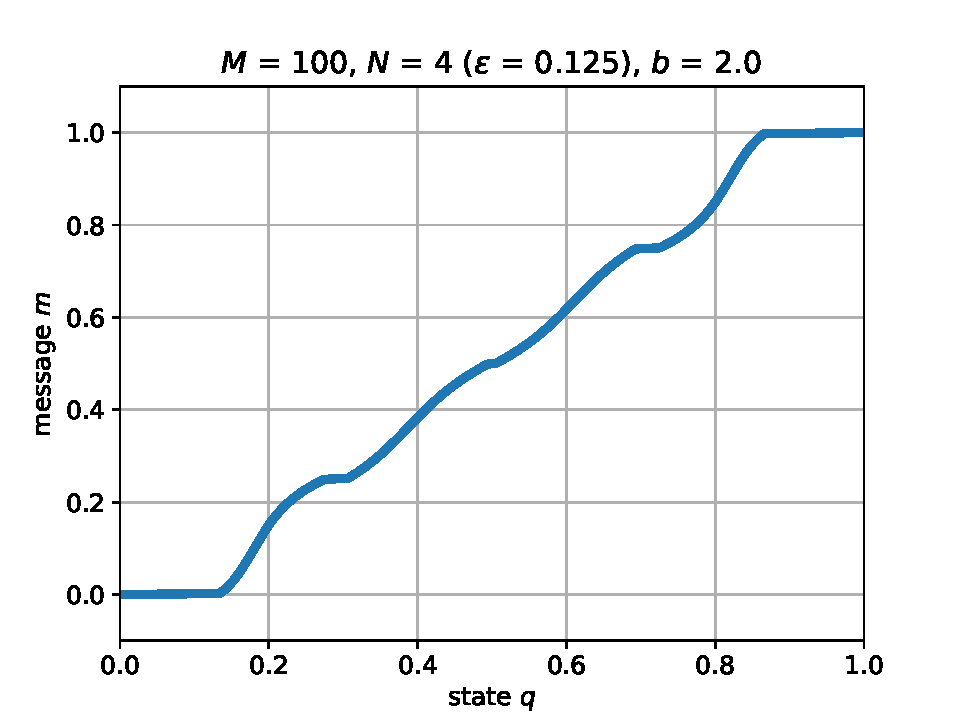
\includegraphics[scale=.5]{msg1} & 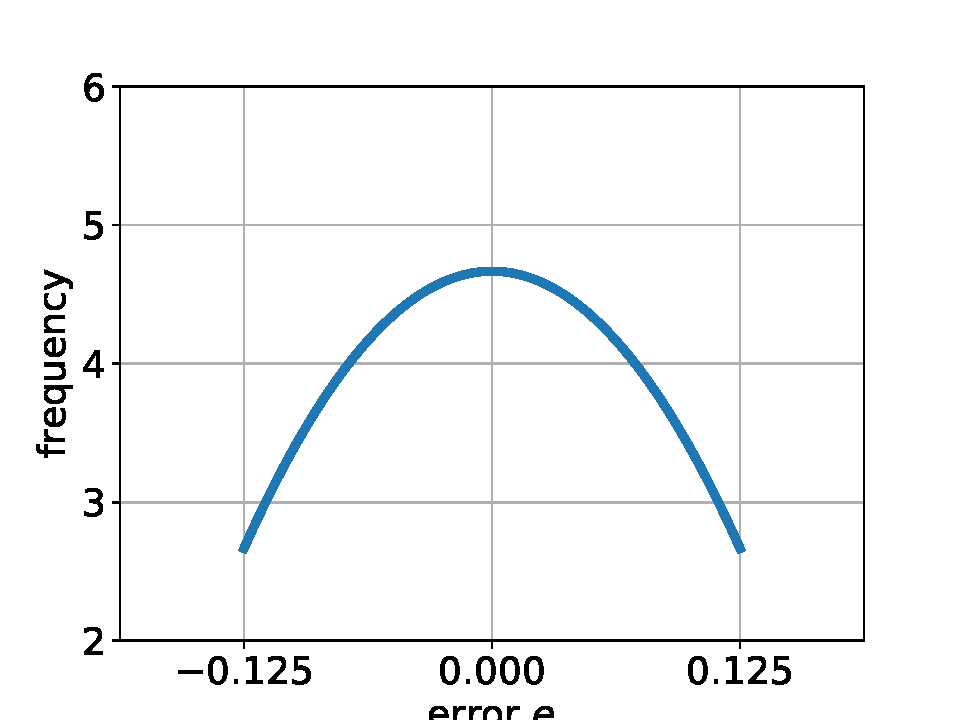
\includegraphics[scale=.5]{err1} \\
			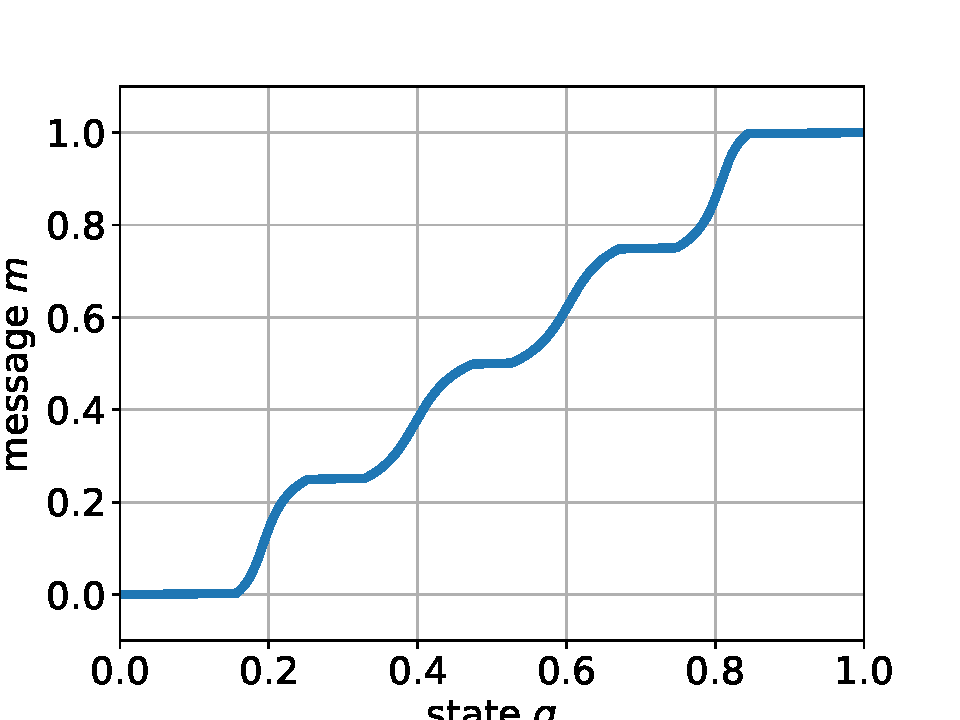
\includegraphics[scale=.5]{msg2} & 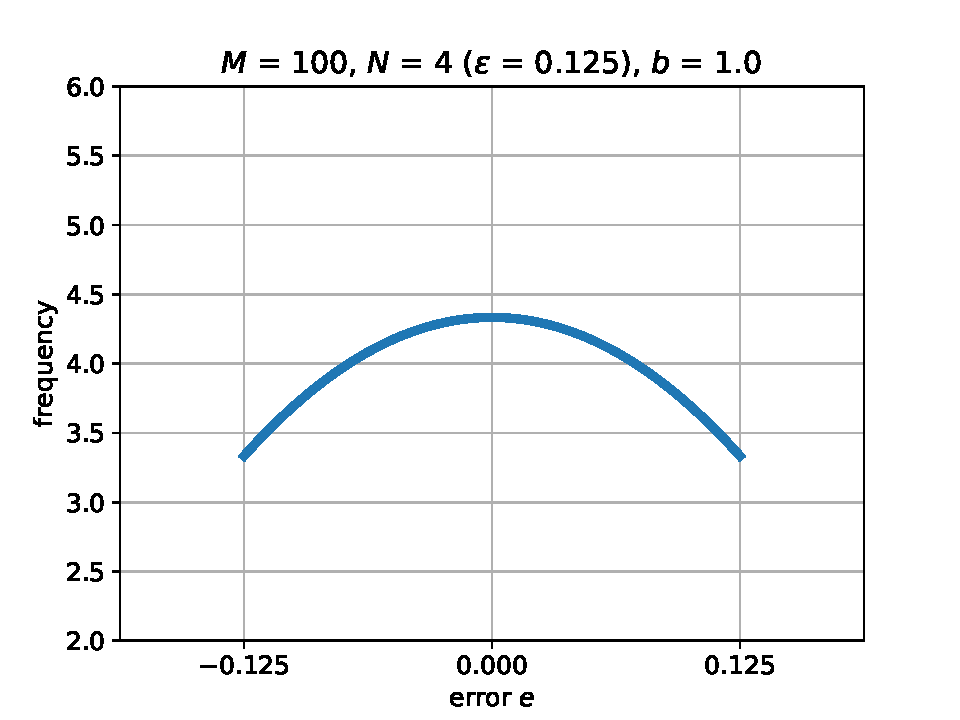
\includegraphics[scale=.5]{err2} \\
			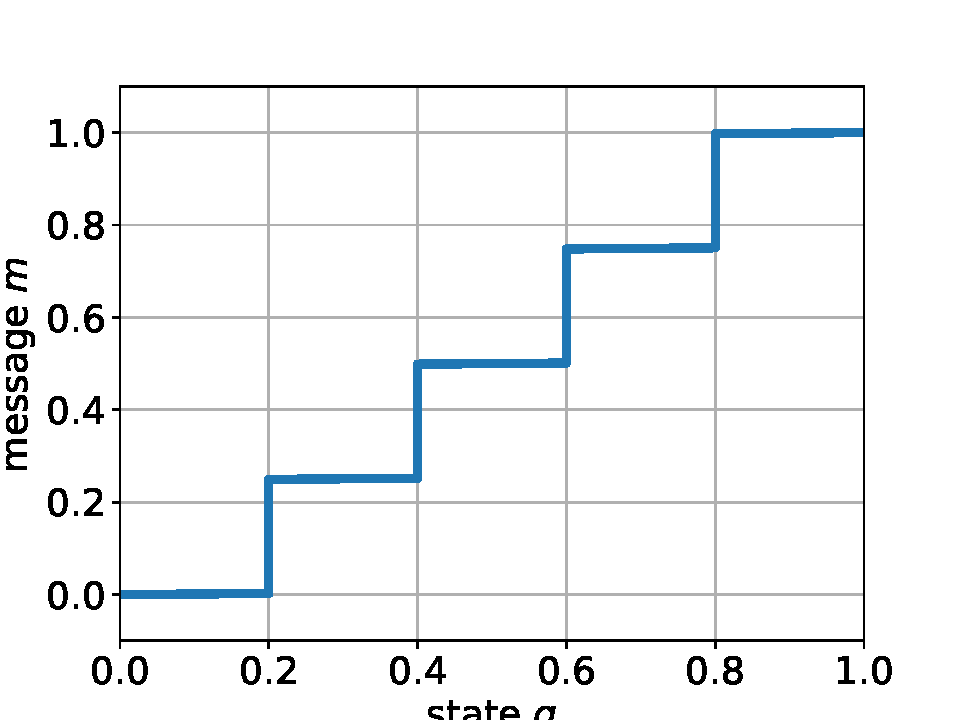
\includegraphics[scale=.5]{msg4} & 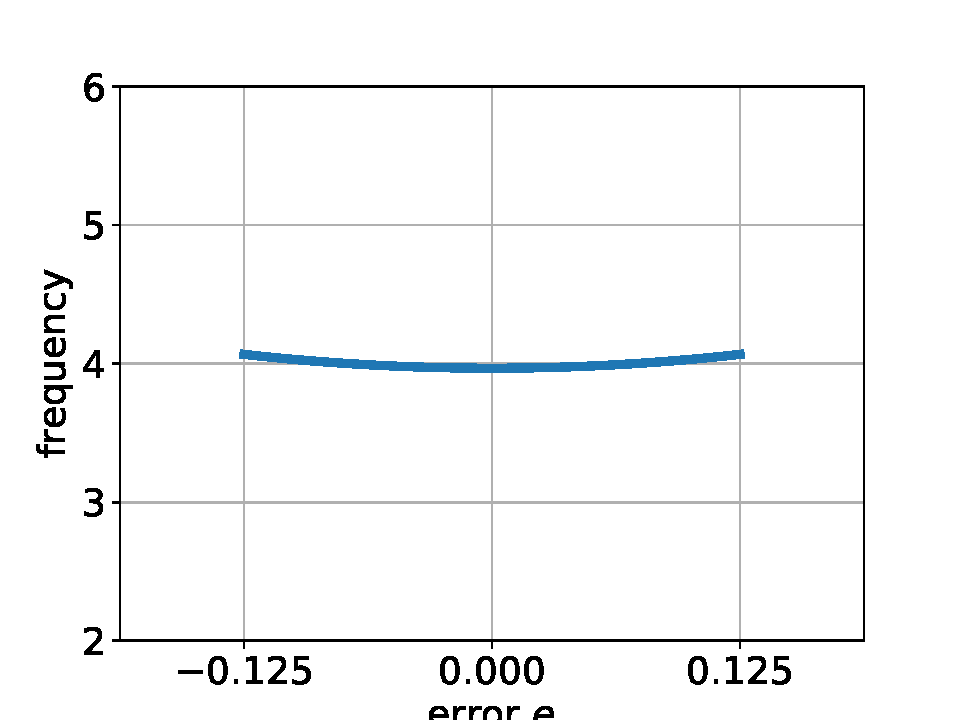
\includegraphics[scale=.5]{err4} \\
			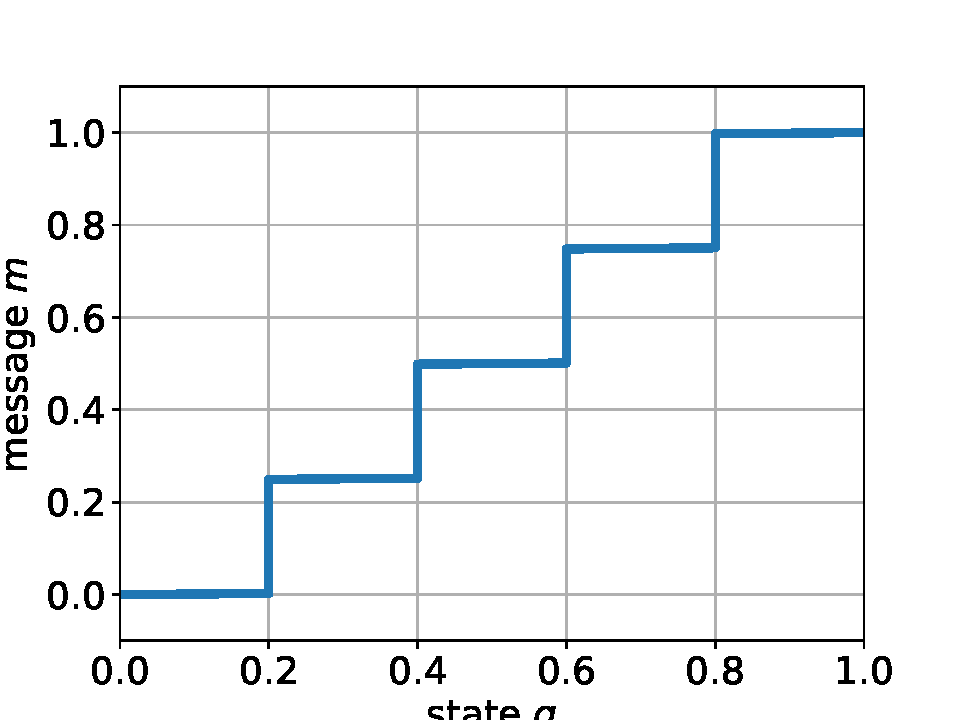
\includegraphics[scale=.5]{msg5} & 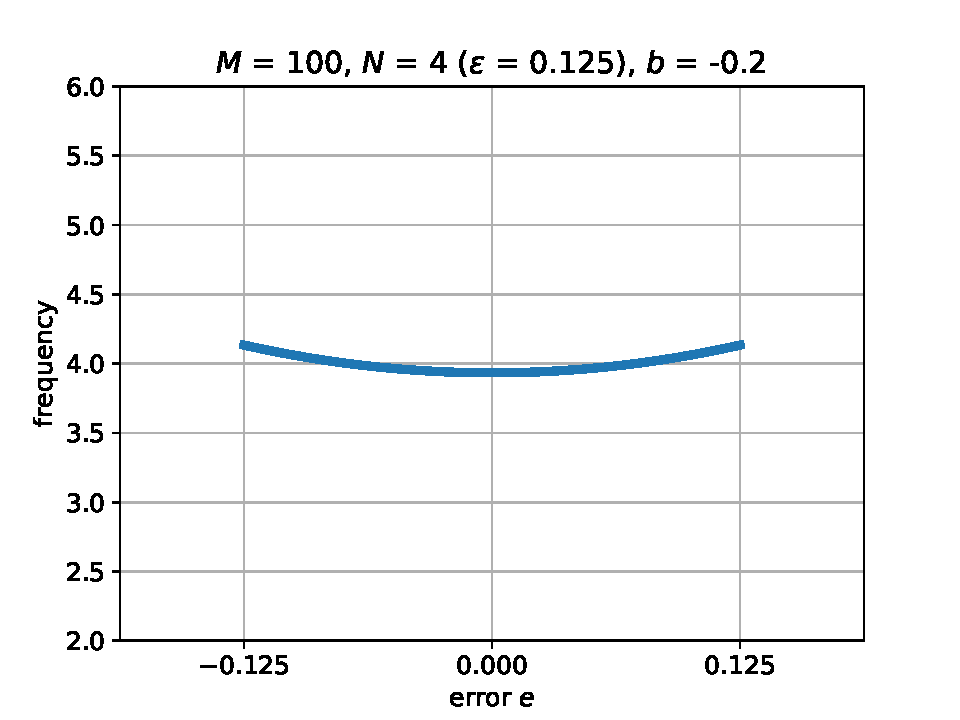
\includegraphics[scale=.5]{err5} 
		\end{tabular}
	\end{center}
\end{figure}
\iffalse
\pagebreak
\begin{landscape}
	\subsection{Example: $A$, $B$, and $C$ when $M=4$ an $N=2$}
	Note that the columns of $A$ are all the same. The same is true for $B$. 
	\tiny
	\begin{align}
		A&=\left[\begin{array}{cccccccccc}
\alpha_{-4,0} &  &  &  &  &  &  &  & \\
\alpha_{-3,0} & \alpha_{-3,1} &  &  &  &  &  &  & \\
\alpha_{-2,0} & \alpha_{-2,1} & \alpha_{-2,2} &  &  &  &  &  & \\
\alpha_{-1,0} & \alpha_{-1,1} & \alpha_{-1,2} & \alpha_{-1,3} &  &  &  &  & \\
 & \alpha_{0,1} & \alpha_{0,2} & \alpha_{0,3} & \alpha_{0,4} &  &  &  & \\
 &  & \alpha_{1,2} & \alpha_{1,3} & \alpha_{1,4} & \alpha_{1,5} &  &  & \\
 &  &  & \alpha_{2,3} & \alpha_{2,4} & \alpha_{2,5} & \alpha_{2,6} &  & \\
 &  &  &  & \alpha_{3,4} & \alpha_{3,5} & \alpha_{3,6} & \alpha_{3,7} & \\
 &  &  &  &  & \alpha_{4,5} & \alpha_{4,6} & \alpha_{4,7} & \alpha_{4,8}\\
 &  &  &  &  &  & \alpha_{5,6} & \alpha_{5,7} & \alpha_{5,8}\\
 &  &  &  &  &  &  & \alpha_{6,7} & \alpha_{6,8}\\
 &  &  &  &  &  &  &  & \alpha_{7,8}
\end{array}\right]\\
		B&=\left[\begin{array}{cccccccc}
\alpha_{-4,0} &  &  &  &  &  &  & \\
\alpha_{-3,0}-\alpha_{-3,1} & \alpha_{-3,1} &  &  &  &  &  & \\
\alpha_{-2,0}-\alpha_{-2,1} & \alpha_{-2,1}-\alpha_{-2,2} & \alpha_{-2,2} &  &  &  &  & \\
\alpha_{-1,0}-\alpha_{-1,1} & \alpha_{-1,1}-\alpha_{-1,2} & \alpha_{-1,2}-\alpha_{-1,3} & \alpha_{-1,3} &  &  &  & \\
-\alpha_{0,1} & \alpha_{0,1}-\alpha_{0,2} & \alpha_{0,2}-\alpha_{0,3} & \alpha_{0,3}-\alpha_{0,4} & \alpha_{0,4} &  &  & \\
 & -\alpha_{1,2} & \alpha_{1,2}-\alpha_{1,3} & \alpha_{1,3}-\alpha_{1,4} & \alpha_{1,4}-\alpha_{1,5} & \alpha_{1,5} &  & \\
 &  & -\alpha_{2,3} & \alpha_{2,3}-\alpha_{2,4} & \alpha_{2,4}-\alpha_{2,5} & \alpha_{2,5}-\alpha_{2,6} & \alpha_{2,6} & \\
 &  &  & -\alpha_{3,4} & \alpha_{3,4}-\alpha_{3,5} & \alpha_{3,5}-\alpha_{3,6} & \alpha_{3,6}-\alpha_{3,7} & \alpha_{3,7}\\
 &  &  &  & -\alpha_{4,5} & \alpha_{4,5}-\alpha_{4,6} & \alpha_{4,6}-\alpha_{4,7} & \alpha_{4,7}-\alpha_{4,8}\\
 &  &  &  &  & -\alpha_{5,6} & \alpha_{5,6}-\alpha_{5,7} & \alpha_{5,7}-\alpha_{5,8}\\
 &  &  &  &  &  & -\alpha_{6,7} & \alpha_{6,7}-\alpha_{6,8}\\
 &  &  &  &  &  &  & -\alpha_{7,8}
\end{array}\right]\\
		C&=\left[\begin{tabular}{cccccccccccccc}
$-\alpha_{-4,0}$ & $\alpha_{-4,0}$ & $0$ & $0$ & $0$ & $0$ & $0$ & $0$ & $0$ & $0$ & $0$ & $0$ & $0$ & $0$\\
$-\alpha_{-3,0}$ & $\alpha_{-3,0}-\alpha_{-3,1}$ & $\alpha_{-3,1}$ & $0$ & $0$ & $0$ & $0$ & $0$ & $0$ & $0$ & $0$ & $0$ & $0$ & $0$\\
$-\alpha_{-2,0}$ & $\alpha_{-2,0}-\alpha_{-2,1}$ & $\alpha_{-2,1}-\alpha_{-2,2}$ & $\alpha_{-2,2}$ & $0$ & $0$ & $0$ & $0$ & $0$ & $0$ & $0$ & $0$ & $0$ & $0$\\
$-\alpha_{-1,0}$ & $\alpha_{-1,0}-\alpha_{-1,1}$ & $\alpha_{-1,1}-\alpha_{-1,2}$ & $\alpha_{-1,2}-\alpha_{-1,3}$ & $\alpha_{-1,3}$ & $0$ & $0$ & $0$ & $0$ & $0$ & $0$ & $0$ & $0$ & $0$\\
$0$ & $-\alpha_{0,1}$ & $\alpha_{0,1}-\alpha_{0,2}$ & $\alpha_{0,2}-\alpha_{0,3}$ & $\alpha_{0,3}-\alpha_{0,4}$ & $\alpha_{0,4}$ & $0$ & $0$ & $0$ & $0$ & $0$ & $0$ & $0$ & $0$\\
$0$ & $0$ & $-\alpha_{1,2}$ & $\alpha_{1,2}-\alpha_{1,3}$ & $\alpha_{1,3}-\alpha_{1,4}$ & $\alpha_{1,4}-\alpha_{1,5}$ & $\alpha_{1,5}$ & $0$ & $0$ & $0$ & $0$ & $0$ & $0$ & $0$\\
$0$ & $0$ & $0$ & $-\alpha_{2,3}$ & $\alpha_{2,3}-\alpha_{2,4}$ & $\alpha_{2,4}-\alpha_{2,5}$ & $\alpha_{2,5}-\alpha_{2,6}$ & $\alpha_{2,6}$ & $0$ & $0$ & $0$ & $0$ & $0$ & $0$\\
$0$ & $0$ & $0$ & $0$ & $-\alpha_{3,4}$ & $\alpha_{3,4}-\alpha_{3,5}$ & $\alpha_{3,5}-\alpha_{3,6}$ & $\alpha_{3,6}-\alpha_{3,7}$ & $\alpha_{3,7}$ & $0$ & $0$ & $0$ & $0$ & $0$\\
$0$ & $0$ & $0$ & $0$ & $0$ & $-\alpha_{4,5}$ & $\alpha_{4,5}-\alpha_{4,6}$ & $\alpha_{4,6}-\alpha_{4,7}$ & $\alpha_{4,7}-\alpha_{4,8}$ & $\alpha_{4,8}$ & $0$ & $0$ & $0$ & $0$\\
$0$ & $0$ & $0$ & $0$ & $0$ & $0$ & $-\alpha_{5,6}$ & $\alpha_{5,6}-\alpha_{5,7}$ & $\alpha_{5,7}-\alpha_{5,8}$ & $\alpha_{5,8}-\alpha_{5,9}$ & $\alpha_{5,9}$ & $0$ & $0$ & $0$\\
$0$ & $0$ & $0$ & $0$ & $0$ & $0$ & $0$ & $-\alpha_{6,7}$ & $\alpha_{6,7}-\alpha_{6,8}$ & $\alpha_{6,8}-\alpha_{6,9}$ & $\alpha_{6,9}-\alpha_{6,10}$ & $\alpha_{6,10}$ & $0$ & $0$\\
$0$ & $0$ & $0$ & $0$ & $0$ & $0$ & $0$ & $0$ & $-\alpha_{7,8}$ & $\alpha_{7,8}-\alpha_{7,9}$ & $\alpha_{7,9}-\alpha_{7,10}$ & $\alpha_{7,10}-\alpha_{7,11}$ & $\alpha_{7,11}$ & $0$\\
$0$ & $0$ & $0$ & $0$ & $0$ & $0$ & $0$ & $0$ & $0$ & $-\alpha_{8,9}$ & $\alpha_{8,9}-\alpha_{8,10}$ & $\alpha_{8,10}-\alpha_{8,11}$ & $\alpha_{8,11}-\alpha_{8,12}$ & $\alpha_{8,12}$\\
$0$ & $0$ & $0$ & $0$ & $0$ & $0$ & $0$ & $0$ & $0$ & $0$ & $-\alpha_{9,10}$ & $\alpha_{9,10}-\alpha_{9,11}$ & $\alpha_{9,11}-\alpha_{9,12}$ & $\alpha_{9,12}$\\
$0$ & $0$ & $0$ & $0$ & $0$ & $0$ & $0$ & $0$ & $0$ & $0$ & $0$ & $-\alpha_{10,11}$ & $\alpha_{10,11}-\alpha_{10,12}$ & $\alpha_{10,12}$\\
$0$ & $0$ & $0$ & $0$ & $0$ & $0$ & $0$ & $0$ & $0$ & $0$ & $0$ & $0$ & $-\alpha_{11,12}$ & $\alpha_{11,12}$
\end{tabular}\right]
	\end{align}
\end{landscape}
\fi
\end{document}
